% Intended LaTeX compiler: pdflatex
\documentclass[10pt,a4paper,UTF8]{article}
\usepackage{zclorg}
\usepackage{tikztheorem}
\author{emacsun}
\date{}
\title{冒泡排序}
\hypersetup{
 pdfauthor={emacsun},
 pdftitle={冒泡排序},
 pdfkeywords={},
 pdfsubject={},
 pdfcreator={Emacs 25.0.50.1 (Org mode 9.0.6)},
 pdflang={English}}
\begin{document}

\maketitle
\tableofcontents
\titlepic{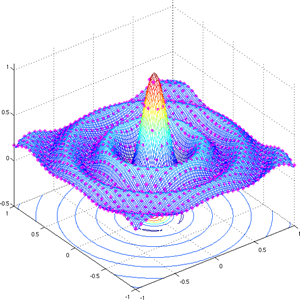
\includegraphics[scale=0.25]{../../img/sinc.PNG}}

\section{算法描述}
\label{sec:org9fbaaa9}


插入排序是一个简单的基于插入的排序算法。当输入的数据规模较小或者输入数据基本已经排好序时,这个算法比较有效。此算法也用来配合其他比较高级的算法完成排序。

可以用这样一个场景来描述插入排序:假设待排序列的数字都印在卡片上,并且卡片叠在一起朝下扣在桌面上。此时你手中没有一张卡片。排序开始,你用右手从桌上揭起一张卡片放到左手中,此时左手中有一张卡片,当然这张卡片是排好序的。接着,你又揭起第二张卡片,此时你比较这张卡片和左手中的卡片。如果新揭起的卡片上数字大于第一次揭起的卡片上数字,就把第二张卡片放在第一张卡片右边,否则就放在左边。依次类推。这样,你左手的卡片始终是排好序的,右手那一张新揭起来的卡片是本次排序需要插入的,桌面上的剩余卡片是还没有来得及排序的。当桌面和右手都没有卡片时,左手的卡片就是全部排好序的卡片。

\section{示例}
\label{sec:org23f3851}


假设输入数据是(5,2,4,6,1,3),图\ref{fig:org1809d32}给出插入排序的排序过程。
\begin{figure}[htbp]
\centering
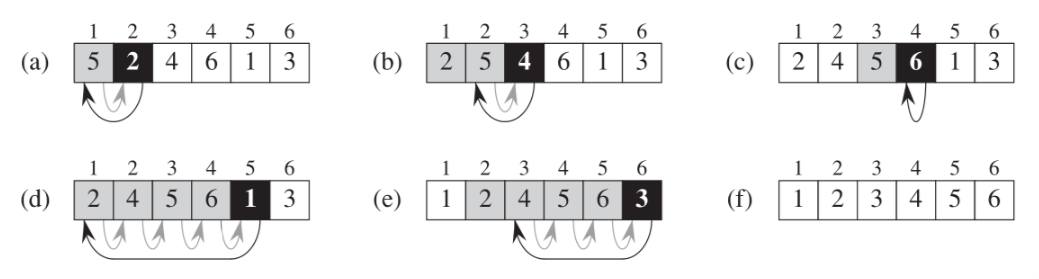
\includegraphics[width=0.6\textwidth]{../../img/computer_algorithms/20170702insertionSort.png}
\caption{\label{fig:org1809d32}
(5,2,4,6,1,3)的插入排序过程}
\end{figure}

\section{插入排序伪代码}
\label{sec:org301b519}


插入排序的伪代码如图\ref{fig:orgc8a3b3b}所示:

\begin{figure}[htbp]
\centering
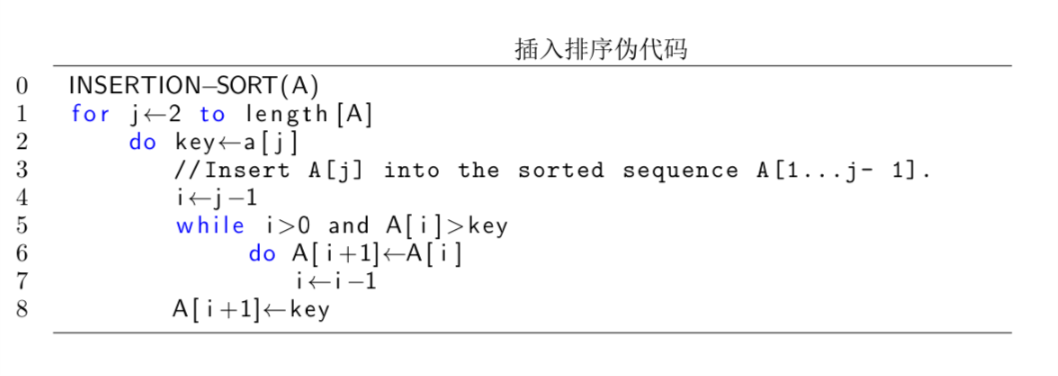
\includegraphics[width=0.6\textwidth]{../../img/computer_algorithms/20170702insertionSortPseudoCode.png}
\caption{\label{fig:orgc8a3b3b}
插入排序伪代码}
\end{figure}
\section{算法分析}
\label{sec:orgdbcae43}


图\ref{fig:org1809d32} 给出(5,2,4,6,1,3)的插入排序过程。在伪代码中,索引\(j\)表示当前在右手中的扑克牌,它将要被插入到左手已经排好序的序列中去。在每一次的外部 \texttt{for} 循环中,有序子序列为\(A[1,\ldots,j-1]\),未排序的序列为\(A[j+1,\ldots,n]\),待排序的元素为\(A[j]\)。我们用循环不变式来陈述\(A[1,\ldots,j-1]\)的一些特性。

在每一次外部 \texttt{for} 循环中,子序列 \(A[1,\ldots,j-1]\) 对应初始已排序列。

\begin{enumerate}
\item Initialization 我们证明,在第一次循环中,即\(j=2\)时,循环不变式成立。这是显然的,当\(j=2\)时,子序列\(A[1,\ldots,j-1]=A[1]\),只有一个元素,当然是成立的。
\item Maintenance 我们证明:在接下来的每一次循环中,循环不变式成立。这是很显然的,每一次我们都移动\(A[j-1],A[j-2],\ldots\)为\(A[j]\)找到合适的位置。这样,下一次 \texttt{for} 循环开始时,子序列 \(A[1,\ldots,j-1]\) 是已经排好的子序列。
\item Termination 最后我们检验当循环结束时排序结果。对于插入排序来说。当\(j > n\)时,排序结束。当\(j=n+1\)时子序列\(A[1,\ldots,n]\)对应已经排好序的子序列,显然这个序列就是我们需要的结果。
\end{enumerate}

以上,我们分析了插入排序的正确性,接下来我们分析插入排序的复杂度。此处我们只分析插入算法的时间复杂度。事实上,一个算法的时间复杂度取决于多种因素,比如输入的数组大小和输入数组的已排序程度。通常来讲一个算法需要的时间随着输入规模的增大而增大。在插入排序中,我们假定伪代码每一行运行需要的时间是固定的,第\(i\)行运行需要时间\(c_i\)。对于每一个\(j=2,3,\ldots,n\),定义\(t_j\)为需要判断 \texttt{while} 循环条件的次数。当 \texttt{for} 循环和 \texttt{while} 循环结束时,判断条件要比循环体多执行一次。最后,我们标记伪代码中每一行需要的时间。

\begin{figure}[htbp]
\centering
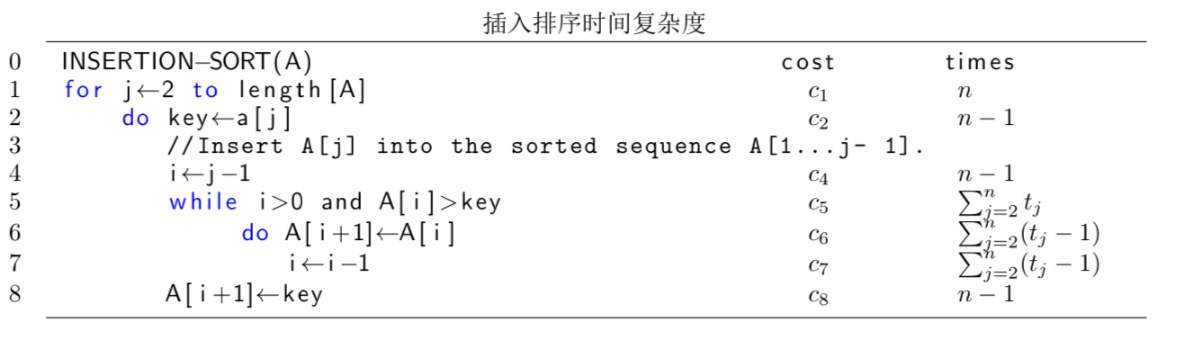
\includegraphics[width=0.6\textwidth]{../../img/computer_algorithms/20170702insertionSortComplexity.png}
\caption{\label{fig:org08ee299}
插入排序的时间复杂度}
\end{figure}


总的运行时间可以表示为:
\begin{equation}
\label{eq:1}
  T(n) = c_1n + c_2(n-1) + c_4(n-1) + c_5\sum_{j=2}^nt_j + c_6\sum_{j=2}^n(t_j-1) + c_7 \sum_{j=2}^n(t_j-1) + c_8(n-1)
\end{equation}

需要注意的是,即使相同规模的输入,也会产生不同的运行时间。对于插入排序,当输入已经排好序时,运行时间最少,此时\(t_j=1,j=2,3,\ldots,n\)。
\begin{equation}
\label{eq:2}
  T(n) = (c_1 + c_2 + c_4 + c_5 + c_8)n - (c_2 + c_4 + c_5 + c_8) = An+B
\end{equation}

如果输入序列是按逆序排好的序列,则运行时间最长。此时\(t_j=j,j=2,3,\ldots,n\)
\begin{equation}
\label{eq:3}
  T(n) = (\frac{c_5}{2} + \frac{c_6}{2} +\frac{c_7}{2} )n^2 + (c_1 + c_2 + c_4+\frac{c_5}{2}- \frac{c_6}{2}-\frac{c_7}{2}+c_8)n -(c_2 + c_4 + c_5 + c_8)
\end{equation}

最差情况可以表述为\(T(n)=An^2+Bn+C\)。

在插入排序的时间复杂度中,我们给出了最好情况和最差情况的复杂度。在以后的分析过程中,我们只分析最差运行时间,也就是对于输入规模为\(n\)的输入的最长运行时间。这样做有三点理由:

\begin{enumerate}
\item 最差运行时间给出了算法运行时间的上界。也即给出了算法运行永远不会超过的时间。
\item 对于一些算法,最差情况经常发生。
\item 平均时间复杂度通常趋近于最差情况,至少在数量级上是相同的。
\end{enumerate}

\section{插入排序C代码实现}
\label{sec:org261650b}

编辑环境:Emacs;编译:GCC;调试:GDB;操作系统:Windows XP SP3;CPU:Intel core i5-2400; memory:3.16GB

\lstset{language=C,label= ,caption= ,captionpos=b,firstnumber=1,numbers=left}
\begin{lstlisting}

int *  insertion_sort (int   a[] )
  {
      int i=0,j=0,key=0;
      for(j=1;j<10;j++)
      {
          key = a[ j ];
          i = j-1;
          while (i>-1 && a[ i ] > key )
          {
              a[ i + 1 ] = a [ i ];
              i--;
          }
          a[ i+1 ] = key;
      }
      return a;
  }
\end{lstlisting}
\end{document}
